%%%%%%%%%%%%%%%%%%%%%%%%%%%%%%%%%%%%%%%%%%%%%%
\section{Collaboration Use Cases: P2P and TE}\label{sec:Oracle-and-TE}
%%%%%%%%%%%%%%%%%%%%%%%%%%%%%%%%%%%%%%%%%%%%%%

The growth of demand for content is motivating collaboration between ISPs and
applications. In this chapter we review to use cases: P2P and Traffic Engineering.

\subsection{Use Case: P2P}\label{sec:oracle} 

Recall, P2P systems are self-organizing systems of autonomous entities, called
peers, that cooperate for common goals. These common goals range from sharing
of resources, e.g., music and video files, processing power, or storage
space~\cite{P2P-LNCS-05} to collaborative routing as in Skype and P2P-TV.  A
fundamental characteristic of these systems is their distributed designs and
resources.

Advantages of P2P systems include elimination of bottlenecks and single
points-of-failure within the system, increased processing power, high
availability/redundancy, and little or no dependence on any particular central
entity.  However, P2P systems are plagued by some fundamental issues, such as
overlay/underlay topological and routing mismatch~\cite{sa-oidronl-06},
inefficiencies in locating and retrieving resources, and scalability and
performance issues caused by uncontrolled traffic swamps~\cite{P2P-LNCS-05}.

Several of these drawbacks can be addressed by collaboration between the P2P
overlay and the Internet routing underlay. To overcome these limits each ISP
can offer the ``oracle'' service as introduced in
Section~\ref{sec:p2p-collaboration} to the P2P users which explicitly helps P2P
users to choose ``good'' neighbors.  The P2P user can supply its ISP's oracle
with a list of possible P2P neighbors, during bootstrapping and/or content
exchange.  The ISP's oracle then returns a ranked list to the querying user,
according to its preference (\eg AS-hop distance) and knowledge of the ISP
topology and traffic volume, while at the same time keeping the interest of the
P2P user in mind.  We  show that in principle, P2P systems as well as the ISPs
profit from the use of the oracle even when only considering the AS-distance
for ranking nodes~\cite{afs-cispp2pcip-ccr07}, because the overlay topology is now
localized and respects the underlying Internet topology, and the P2P user
profits from the ISP's knowledge.

To study the impact of biased neighbor selection on a real P2P network that
implements its own routing, we run extensive simulations of the Gnutella
protocol. We show that in contrast to the unmodified P2P system, the ISP-aided
localized P2P system shows consistent improvements in the observed end-user
experience, measured in terms of content download times, network locality of
query responses and desired content, and quality of query responses. A
significantly large portion of P2P traffic remains local to the ISP network,
and ISPs notice a substantial reduction in overall P2P traffic. This can lead
to immense cost savings for the ISPs~\cite{Cachelogic}. The oracle consistently
shows performance gains even across different topologies under a broad range of
user behavior scenarios. For a more detailed analysis of the P2P oracle
service, see~\cite{afs-cispp2pcip-ccr07, af-ispabqsp2pt-eccs07,afk-icsecispp2p-icin07}.



\subsubsection{Influence on P2P Topology}\label{sec:Influence-Oracle-on-P2P-Topology}

To explore the influence of consulting the oracle on the network topology we
visualize, in Figure~\ref{fig:oracle:gnutella_topology}~\cite{tashev-thesis},
the Gnutella overlay topology. At a particular instant in time, we sample the
Gnutella overlay topology, display all the online nodes in the graph, and join
two nodes with an edge if there exists a Gnutella peering between them at this
point of time. The resulting graph structures are displayed in
Figure~\ref{fig:oracle:gnutella_topology}. For our simulations we consider $5$
different topologies: Germany, USA, World1, World2 and World3, each modeled
after their respective AS topologies (World1-3 differ in the size of the ASes).
We can easily observe that the Gnutella topology in the biased case is well
correlated with the Internet AS topology, where the nodes within an AS form a
dense cluster, with only a few connections going to nodes in other ASes. This
is in stark contrast to the unbiased Gnutella graph, where no such property can
be observed. Multiple runs of the above experiments, using the different
topologies yield similar results.

\begin{figure}[tbp]
   \begin{subfigure}[]{0.4\linewidth}
     {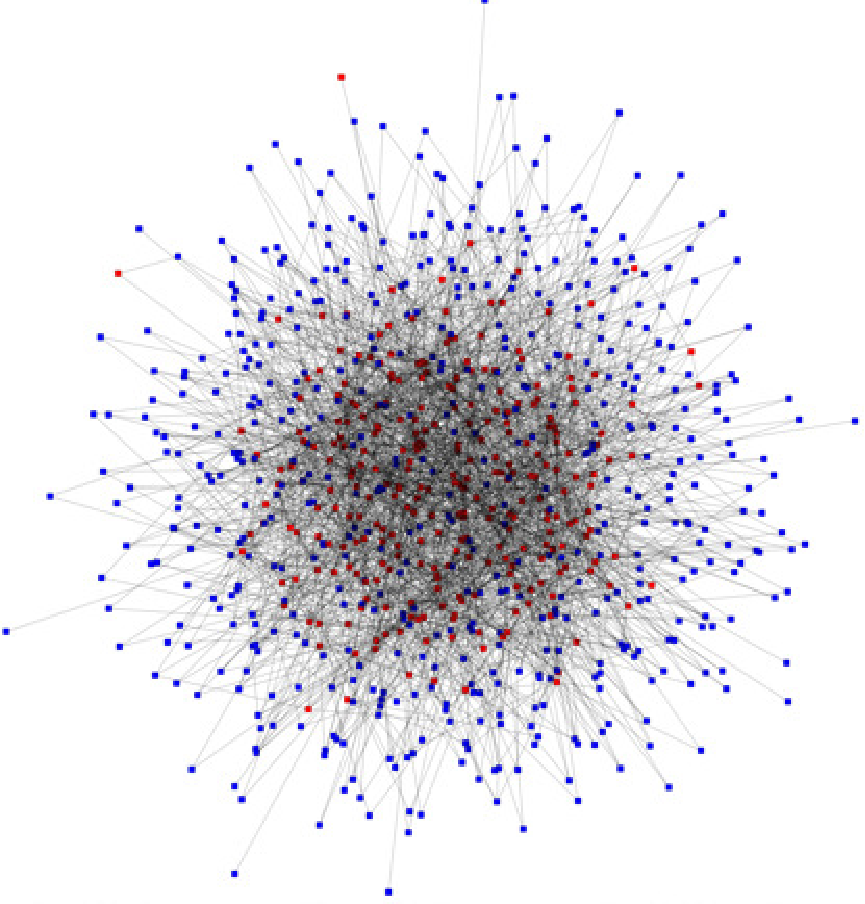
\includegraphics[angle=-90,width=1\linewidth]{figures-pdf/snapshot_nond}}
   \caption{Unbiased Gnutella}%
   \end{subfigure}
\hfill
   \begin{subfigure}[]{0.45\linewidth}
     {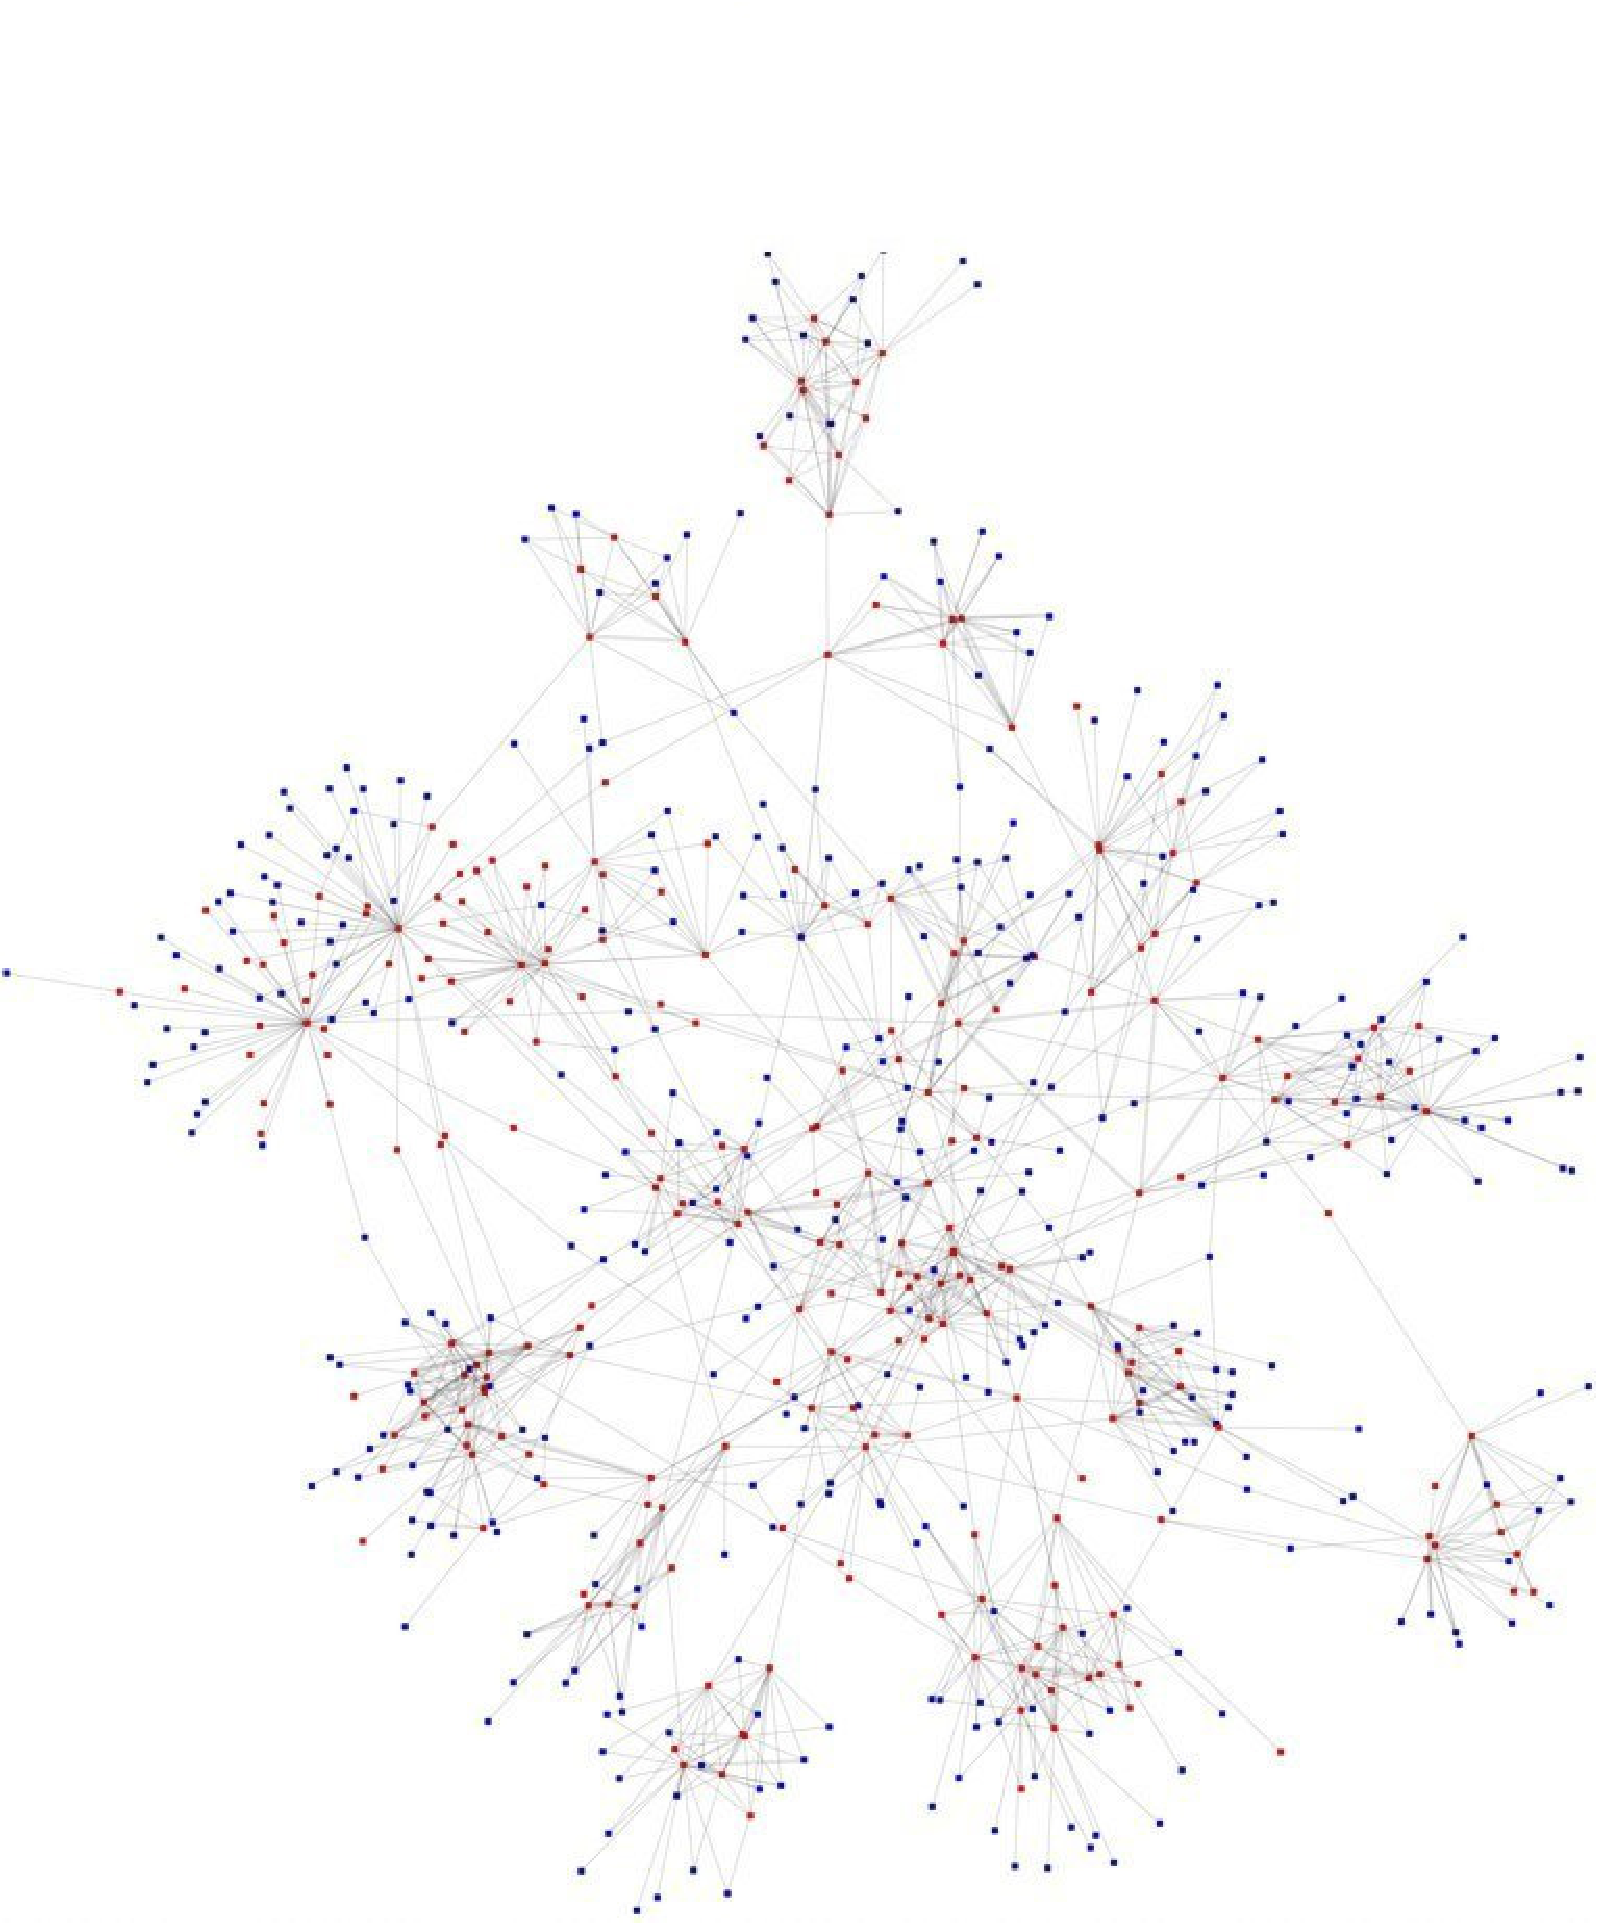
\includegraphics[angle=-90,width=1\linewidth]{figures-pdf/snapshot_nd}}
   \caption{Gnutella with Oracle}%
   \end{subfigure}   \caption{Visualization of Gnutella
     overlay topology. Reprinted from \cite{afs-cispp2pcip-ccr07}. Included here by permission.}
   \label{fig:oracle:gnutella_topology}
\end{figure}




\subsubsection{Benefits of Collaboration}\label{sec:Benefits-Collaboration-P2P-results}


\noindent\textbf{Mean AS distance:} \\
The benefits of using an oracle for biasing the neighborhood in Gnutella are visible in
Figure~\ref{fig:oracle:gnutella_metric:2a}, which shows the average AS distance (in the underlay)
between any two connected Gnutella nodes. The AS distance is obtained as follows. We map
each Gnutella node's IP address to its parent AS, and for each overlay edge, we find the
network distance in AS hops between the two end-nodes.  We observe that the least amount
of decrease in the average AS distance occurs from $1.93$ to $0.8$ at $1000$ seconds, and
the maximum decrease from $1.94$ to $0.25$ happens at $5000$ seconds. Given that the AS
diameter remains constant at $4$ hops, the average decrease of $1.45$ in the AS distance
is significant. Besides, as the average AS distance in the case of oracle list size of
$1000$ is $0.45$, a value less than $1$, it implies that most of the Gnutella peerings are
indeed within the ASes, i.e., they are not crossing AS boundaries. This can be a major
relief for ISPs, as they do not incur any additional cost for traffic within their
domains. Also traffic that does not leave the network is easier to manage. Moreover, P2P
traffic will not encounter inter-ISP bottlenecks.


\begin{figure}[tbp]
	\begin{subfigure}[]{0.32\linewidth}
     {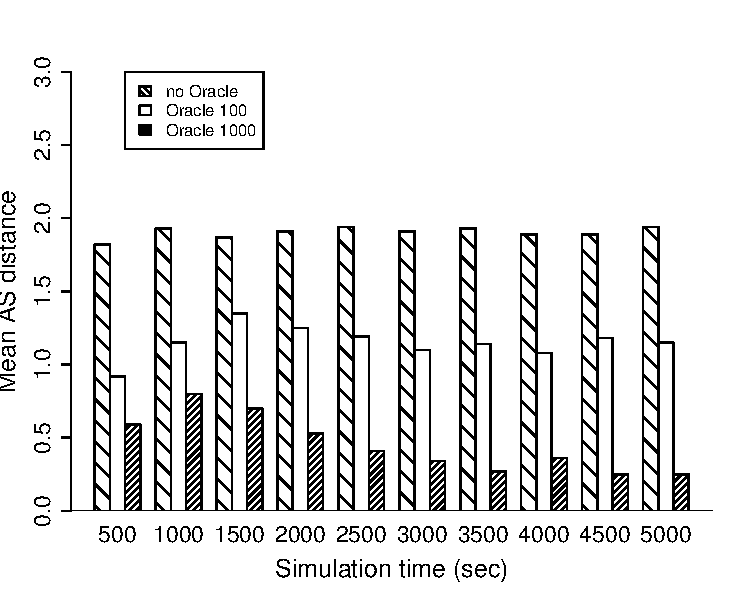
\includegraphics[width=1\textwidth]{figures-pdf/asdist}}
    \caption{Mean AS distance in Underlay\label{fig:oracle:gnutella_metric:2a}}
    \end{subfigure}
 \hfill
    \begin{subfigure}[]{0.32\linewidth}
    {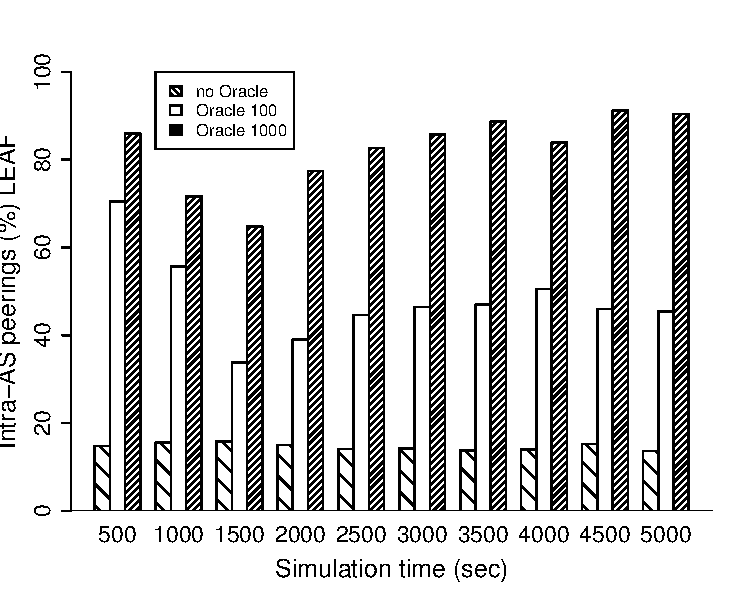
\includegraphics[width=1\textwidth]{figures-pdf/intraAS-leaf}}
    \caption{Intra-AS peerings (\%) for Leaf nodes\label{fig:oracle:gnutella_metric:2b}}
    \end{subfigure}
 \hfill
    \begin{subfigure}[]{0.32\linewidth}
    {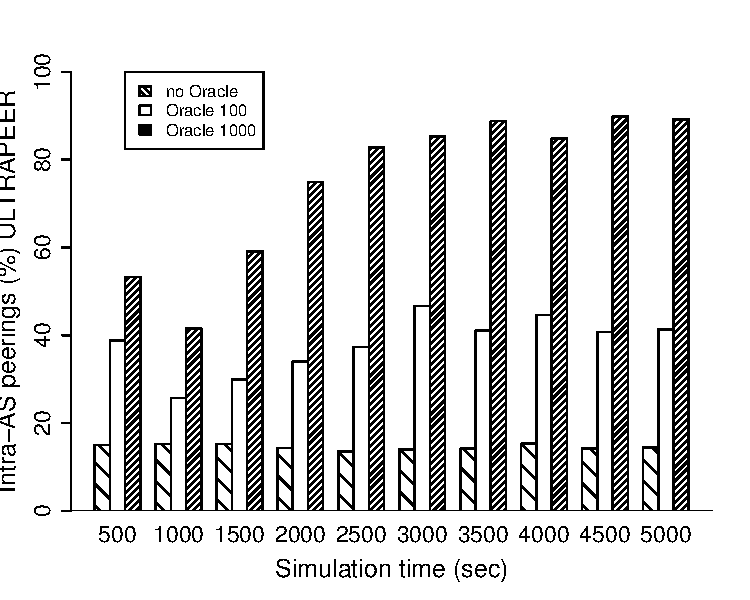
\includegraphics[width=1\textwidth]{figures-pdf/intraAS-up}}
    \caption{Intra-AS peerings (\%) for Ultrapeers\label{fig:oracle:gnutella_metric:2c}}
    \end{subfigure}
    \caption{Metrics for Gnutella simulations}
   \label{fig:oracle:gnutella_metric}
\end{figure}


\vspace{0.75\baselineskip}
\noindent\textbf{Intra-AS P2P connections:} \\
The above observations on AS distance are even better understood from the plots in
Figures~\ref{fig:oracle:gnutella_metric:2b} and \ref{fig:oracle:gnutella_metric:2c}, where we show the total number of intra-AS
P2P connections in the Gnutella network as a percentage of the total number of intra- and
inter-AS P2P connections, for both leafs and ultrapeers.

In Figure~\ref{fig:oracle:gnutella_metric:2b}, we observe that in the case of leaf nodes, taking
the average over the $10$ time points, the percentage of intra-AS P2P connections
increases from $14.6$\% in unbiased case to $47.88$\% in the case of oracle with list size
$100$. For oracle with list size $1000$, we note an average of $82.22$\% intra-AS P2P
connections.

In Figure~\ref{fig:oracle:gnutella_metric:2c}, we observe similar results for ultrapeers. The
percentage of intra-AS P2P connections increases from an average value of $14.54$\% in the
unbiased case to $38.04$\% in the case of oracle with list size $100$, and further to
$74.95$\% in case of oracle with list size $1000$.

The percentage increase in intra-AS P2P connections is larger for leaf nodes as compared
to ultrapeers, a welcome development.  One needs a certain number of inter-AS connections,
to maintain network connectivity and to be able to search for file content that may not be
available within an AS. However, as leaf nodes typically have poor connectivity to the
Internet, and have lower uptimes, it is reasonable to have leaf nodes keep most of their
peerings within their AS, while allowing the ultrapeers to have slightly more connections
outside their ASes.

For the impact of Oracle on download time under different topologies we refer
the reader to~\cite{improving-oracle-GI-2008}. For the impact of Oracle-like
localization techniques on the inter-AS traffic flow of the BitTorrent P2P
system we refer the reader to~\cite{DeepDiving,LocalityP2P,BlindMiceBT,Impact-Profitability}.


%%%%%%%%%%%%%%%%%%%%%%%%%%%%%%%%%%%%%%%%%%%%%%
\subsection{Use Case: Traffic Engineering}\label{sec:te-cate}
%%%%%%%%%%%%%%%%%%%%%%%%%%%%%%%%%%%%%%%%%%%%%%

The growth of demand for content and the resulting deployment of content
delivery infrastructures pose new challenges to CDIs and to ISPs. For CDIs, the
cost of deploying and maintaining such a massive infrastructure has
significantly increased during the last years~\cite{AkamaiCutting:2009} and the
revenue from delivering traffic to end-users has decreased due to the intense
competition. Furthermore, CDIs struggle to engineer and manage their
infrastructures, replicate content based on end-user demand, and assign users
to appropriate servers.

The latter is challenging as end-user to server assignment is based on
inaccurate end-user location
information~\cite{Precise:Mao2002,DNS-extension-IP-client}, and inferring the
network conditions within an ISP without direct information from the network is
difficult. Moreover, due to highly distributed server deployment and adaptive
server assignment, the traffic injected by CDIs is volatile. For example, if
one of its locations is overloaded, a CDI will re-assign end-users to other
locations, resulting in large traffic shifts in the ISP network within minutes.
Current traffic engineering by ISP networks adapts the routing and operates on
time scales of several hours, and is therefore too slow to react to rapid
traffic changes caused by CDIs.

The pressure for cost reduction and customer satisfaction that both CDIs and
ISPs are confronted with, coupled with the opportunity that distributed server
infrastructures offer, motivate us to propose a new tool in the traffic
engineering landscape. We introduce \emph{Content-aware Traffic Engineering}
(\cate). \cate leverages the location diversity offered by CDIs and, through
this, it allows to adapt to traffic demand shifts. In fact, \cate relies on the
observation that by selecting an appropriate server among those available to
deliver the content, the path of the traffic in the network can be influenced
in a desired way. Figure~\ref{fig:flowSelection} illustrates the basic concept
of \cate. The content requested by the client is in principle available from
three servers (A, B, and C) in the network. However, the client only connects
to one of the network locations. Today, the decision of where the client will
connect to is solely done by the CDI and is partially based on measurements
and/or inference of network information and end-user location. With \cate the
decision on end-user to server assignment can be done jointly between the CDI
and ISP.

\begin{figure}[tbp]
  \center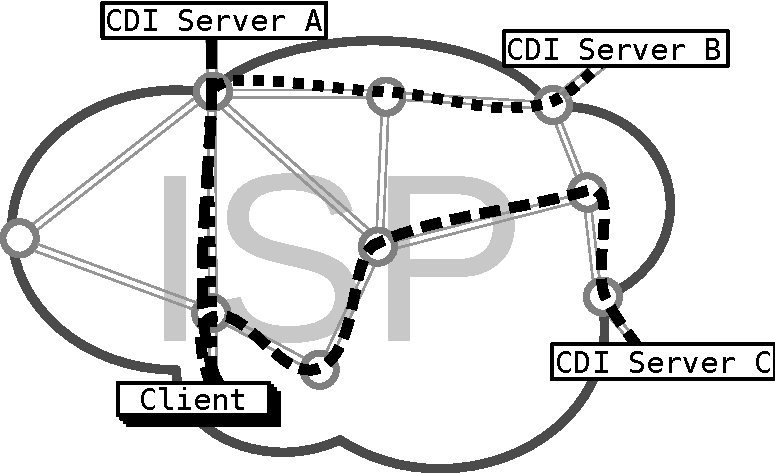
\includegraphics[width=0.8\linewidth]{figures-pdf/trafficShift-concept}
  \caption{By choosing a CDI server for a client with the help of CaTE, traffic
  engineering goals and accurate end-user server assignment become
  possible. Reprinted from \cite{Cate-CCR}. Included here by permission.}
  \label{fig:flowSelection}
  \vspace{-1.5em}
\end{figure}


%%%%
\subsubsection{The CaTE Approach}\label{sec:cate}
%%%%

\cate complements existing traffic engineering solutions
\cite{ietf-alto-protocol,TECDN,CooperativeISPCDN,BeyondMLU,CooperativeISPCDN:Workshop,p4p}
by focusing on traffic demands rather than routing.  Let {\bf y} be the vector
of traffic counts on links and {\bf x} the vector of traffic counts in
origin-destination (OD) flows in the ISP network.  Then {\bf y}=$A${\bf x},
where $A$ is the routing matrix. $A_{ij}=1$ if the OD flow $i$ traverses link
$j$ and $0$ otherwise.  Traditional traffic engineering is the process of
adjusting $A$, given the OD flows {\bf x}, so as to influence the link traffic
{\bf y} in a desirable way.  In \cate, we revisit traffic engineering by
focusing on traffic demands rather than routing changes. Content-aware Traffic
Engineering (\cate) is thus the process of adjusting the traffic demand vector
{\bf x}, without changing the routing matrix $A$, so as to change the link traffic {\bf y}
in a desirable way.

\cate offers additional traffic engineering capabilities to both ISPs and CDNs
to better manage the volatility of content demand in small time scales.
Traditional traffic engineering
\cite{ietf-alto-protocol,TECDN,CooperativeISPCDN,BeyondMLU,CooperativeISPCDN:Workshop,p4p}
relies on changes of routing weights that take place in the time scale of hours
\cite{FT01}.  On the contrary, in \cate, the redirection of end-users to servers can take place
per request or within the TTL of a DNS query that is typically tens of seconds
in large CDNs \cite{PADIS2010}.  Thanks to the online recommendations by ISP
networks, CDNs gain the ability to better assign end-users to servers and
better amortize the deployment and maintenance cost of their infrastructure.
Network bottlenecks are also circumvented and thus the ISP operation is
improved.  Furthermore, the burden of measuring and inferring network topology,
and the state of the network, both challenging problems, is removed from the
CDNs. Moreover, in \cite[Sections 4 and 5]{CaTE-TR} we show that the online
\cate decisions on the end-user to server assignment leads to optimal traffic
assignment within the network under a number of different metrics.  The
advantage is that now the problem of assigning traffic to links reduces to a
fractional solution (on the contrary, assigning routing weights to links is
NP-hard).  In short, all involved parties, including the end-users, benefit
from \cate, creating a win-win situation for everyone.




%%%%%%%%%%%%%%%%%%%%%%%%%%%%%%%
\subsubsection{A Prototype to Support CaTE}\label{sec:system}
%%%%%%%%%%%%%%%%%%%%%%%%%%%%%%%
\cate relies on a close collaboration between CDN and ISP in small time scales
(seconds or per request).  To achieve this goal, network information has to be
collected and processed by the ISP.  Candidate CDN servers have to be
communicated to the ISP and ranked based on a commonly agreed criteria, \eg to
optimize the delay between the end-user and the CDN server.  Today, there is no
system to support the above operations.  This motivate us to design, implement
and evaluate a novel and scalable system that can support \cate.  In this
section we describe the architecture and deployment of our working prototype to
enable \cate.  We start by presenting our prototype in
Section~\ref{sec:architecture}.  We then  comment on its operation and
deployment within the ISP, its interaction with a CDN, and its performance that
is beyond the state-of-the-art \cite{ietf-alto-protocol}.


%%%%%%%%%%%%%%%%%%%%%%%%%%%%%%%%%%%%%%%%%%%%%%%%%%%%%%%%
\ \\\noindent\textbf{Architecture:}\label{sec:architecture}\\\noindent
%%%%%%%%%%%%%%%%%%%%%%%%%%%%%%%%%%%%%%%%%%%%%%%%%%%%%%%
The \cate system is installed in an ISP and interacts with the existing CDN
server selector. The main tasks of the \cate system are to: (1) maintain an
up-to-date annotated map of the ISP network and its properties, (2) produce
preference rankings based on the paths between end-users and candidate servers,
and (3) communicate with the CDN server selection system to influence the
assignment of end-user to servers.  To this end, we propose an architecture
that comprises a {\it Network Monitoring} component, a {\it Query Processing}
component and a {\it communication interface} between an ISP and a CDN.  For an
overview of the architecture see Figure~\ref{fig:CaTE-architecture}.


%%%%%%%%%%%%%%%%%%%%%%%%%%%%%%%%%%%%%%%%%%%%%%%%%%%%%%%%
\ \\\noindent\textbf{Network Monitoring:}\label{sec:Network-monitoring}\\\noindent
%%%%%%%%%%%%%%%%%%%%%%%%%%%%%%%%%%%%%%%%%%%%%%%%%%%%%%%
The network monitoring component gathers information about the topology and the
state of the network from several sources to maintain an up-to-date view of the
network.  The network monitoring component consists of the following
subcomponents:

The {\bf Topology Information} component gathers detailed information about the
basic network topology, \ie routers and links, as well as annotations such as
link utilization, router load, and topological changes.  An Interior Gateway
Protocol (IGP) listener provides up-to-date link-state (\ie IS-IS, OSPF)
information.  Information about routers and links is retrieved, thus, the
network topology can be extracted.  The nominal link delay, \ie the latency on
a link without queuing, can be found through the link length and physical
technology.  The link utilization and other metrics can be retrieved via SNMP
from the routers or an SNMP aggregator.

The {\bf Connectivity Information} component uses routing information to
calculate the paths that traffic takes through the network. Finding the path of
egress traffic can be done by using a Border Gateway Protocol (BGP) listener.
Ingress points of traffic into the ISP network can be found by utilizing
Netflow data. This allows for complete forward and reverse path mapping inside
the ISP.  Furthermore, the system can map customers as well as CDN
infrastructures into the network map by finding the routers that announce the
address space associated with them. In total, this allows for a complete path
map between any two points in the ISP network.  Finally, our system has access
to an uplink database that provides information about the connectivity
statistics of end-users.


\begin{figure}[tbp]
    \center 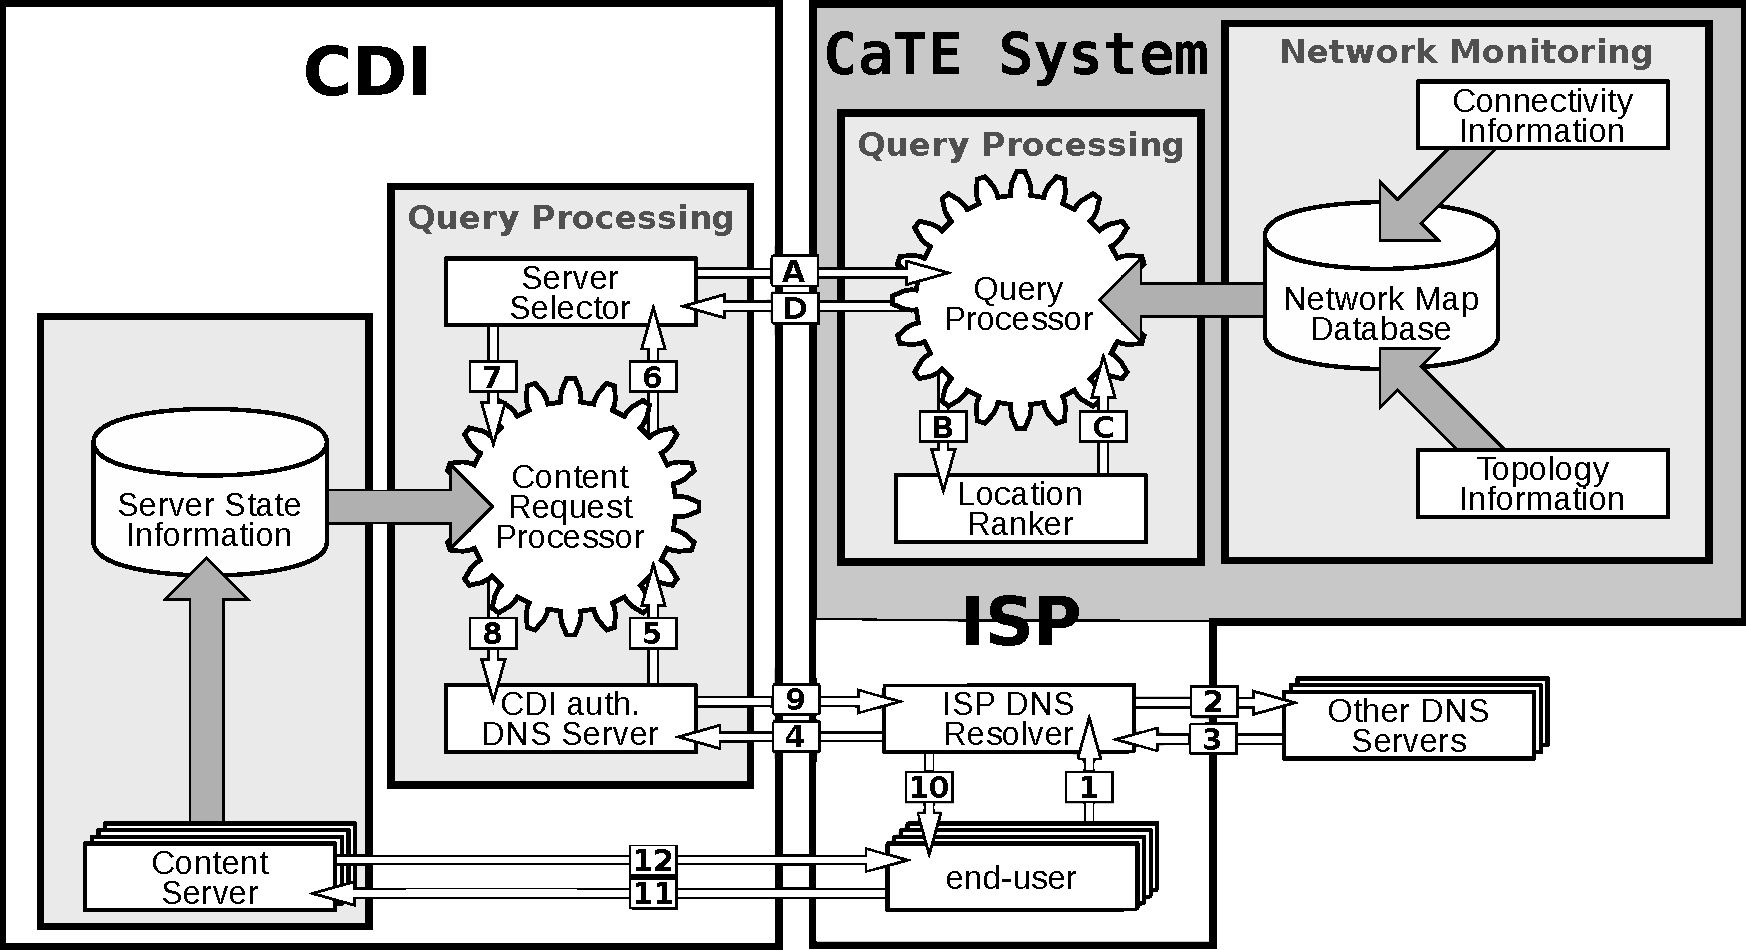
\includegraphics[width=3.2in]{figures-pdf/CaTE_Schematic}
  \vspace{-0.1in}
    \caption{CaTE System architecture and flow of messages. Reprinted from \cite{Cate-CCR}. Included here by permission.}
    \label{fig:CaTE-architecture}
    \vspace{-0.2in}
\end{figure}

The {\bf Network Map Database} component processes the information collected by
the {\it Topology} and {\it Connectivity Information} components to build an
annotated network map of the ISP network tailored towards fast lookup on path
properties.  It uses a layer of indirection to keep the more volatile
information learned from BGP separate from the slower changing topological
information.  This allows address space to be quickly reassigned without any
reprocessing of routing or path information.  It also enables pre-calculation
of path properties for all paths that yields a constant database lookup
complexity independent of path length and network architecture.  If topology
changes, \eg IGP weights change or a link fails, the {\it Topology Information}
component immediately updates the database which only recalculates the
properties of the affected paths.  Having ISP-centric information ready for
fast access in a database ensures timely responses and high query throughput.



%%%%%%%%%%%%%%%%%%%%%%%%%%%%%%%%%%%%%%%%%%%%%%%%%%%%%%%%
\ \\\noindent\textbf{Query Processing:}\label{sec:Query-Processing}\\\noindent
%%%%%%%%%%%%%%%%%%%%%%%%%%%%%%%%%%%%%%%%%%%%%%%%%%%%%%%
The {\bf Query Processing} component receives a description of a request for
content from the CDN, which specifies the end-user making the request and a
list of candidate CDN servers.  It then uses information from the {\it Network
  Map Database} and a selected ranking function to rank the candidate servers.
This component consists of the following subcomponents:

The {\bf Query Processor} receives the query from the CDN.  First, the query
processor maps each source-destination (server to end-user) pair to a path in
the network.  In most cases, the end-user is seen as the ISP DNS resolver,
unless both ISP and CDN support the client IP eDNS
extension~\cite{DNS-extension-IP-client}.  Once the path is found, the
properties of the path are retrieved. Next, the pairs are run individually
through the location ranker subcomponent (see below) to get a preference value.
Finally, the list is sorted by preference values, the values are stripped from
the list, and it is sent back to the CDN.

The {\bf Location Ranker} component computes the preference value for
individual source-destination pairs based on the source-destina\-tion path
properties and an appropriate function.  Which function to use depends on (a)
the CDN, (b) what metrics the CDN asked for and (c) the optimization goal of
the ISP.  The preference value for each source-destination pair is then handed
back to the Query Processor.  Multiple such optimization functions being
defined upon the collaboration agreement and subsequently selected individually
in each ranking request. For example, a function might be the minimization of
end-user and server delay.  In~\cite{CaTE-TR} we evaluate \cate
with multiple ranking functions for different optimization goals.


%%%%%%%%%%%%%%%%%%%%%%%%%%%%%%%%%%%%%%%%%%%%%%%%%%%%%%%%
\ \\\noindent\textbf{Communication Interfaces:}\label{sec:Communication-interfaces}\\\noindent
%%%%%%%%%%%%%%%%%%%%%%%%%%%%%%%%%%%%%%%%%%%%%%%%%%%%%%%
When a CDN receives a content request, the {\it Server Selector} needs to
choose a content server to fulfill this request. We propose that the server
selector sends the list of eligible content servers along with the source of
the query and an optimization goal to the ISP's \cate system to obtain
additional guidance about the underlying network.  If the guidance is at
granularity of a single DNS request, we propose a DNS-like protocol using UDP
to prevent extra overhead for connection management.  If the granularity is at
a coarser level, \ie seconds or even minutes, we rely on TCP.


%%%%%%%%%%%%%%%%%%%%%%%%%%%%%%%%%%%%%%%%%%%%%%%%%%%%%%%%%%%%%%%%%%%%%%
\subsubsection{Privacy and Performance}\label{sec:discussion}
%%%%%%%%%%%%%%%%%%%%%%%%%%%%%%%%%%%%%%%%%%%%%%%%%%%%%%%%%%%%%%%%%%%%%%
During the exchange of messages, none of the parties is revealing any sensitive
operational information.  CDNs only reveal the candidate servers that can
respond to a given request without any additional operational information (\eg
CDN server load, cost of delivery or any reason why a server is chosen). The
set of candidate servers can be updated per request or within a TTL that is
typically in the order of a tens of seconds in popular CDNs \cite{PADIS2010}.
On the other side, the ISP does not reveal any operational information or the
preference weights it uses for the ranking. In fact, the ISP only re-orders a
list of candidate servers provided by the CDN.  This approach differs
significantly from \cite{ietf-alto-protocol,p4p}, where partial or complete
ISP network information, routing weights, or ranking scores are publicly
available.  We argue that an important aspect to improve content delivery is to
rely on up-to-date information during server selection of the CDN.  This also
eliminates the need of CDNs to perform active measurements to infer the
conditions within the ISP that can add overhead to CDN operation and may be
inaccurate.  With \cate, the final decision is still made by the CDN, yet it is
augmented with up-to-date network guidance from the ISP.

To improve the performance of our system, we do not rely on XML-based network
maps as proposed in~\cite{ietf-alto-protocol}, but on light protocols that are
close to DNS in design.  This design choice is important as topology
information in large networks (in the order of multiple MBytes). Transferring
this information periodically to many end-users is likely to be challenging. In
a single instance of our system, we manage to reply to up to $90,000$
queries/sec when 50 candidate servers supplied by the CDN. At this level, the
performance of our system is comparable to that of current DNS servers, such as
BIND. However, the number of replies drops to around $15,000$ per second when
considering $350$ candidate servers. The additional response time when our
system is used is around $1$ ms when the number of candidate servers is $50$
and around $4$ ms when considering $350$ candidate servers. This overhead is
small compared to the DNS resolution time~\cite{DNS-IMC-2010}. The performance
was achieved on a commodity dual-quad core server with 32 GB of RAM and 1GBit
Ethernet interfaces. Furthermore, running additional servers does not require
any synchronization between them.  Thus, multiple servers can be located in
different places inside the network.


%%%%%%%%%%%%%%%%%%%%%%%%%%%%%%%%%%%%%%%%%%%%%%%%%%%%%%%%
\ \\\noindent\textbf{Deployment:}\label{sec:deployment:}\\\noindent
%%%%%%%%%%%%%%%%%%%%%%%%%%%%%%%%%%%%%%%%%%%%%%%%%%%%%%%
Deploying the system inside the ISP network does not require any change in the
network configuration or ISP DNS operation.  Our system solely relies on
protocol listeners and access to ISP network information. Moreover, no
installation of special software is required by end-users.  The \cate system
adds minimal overhead to ISPs and CDNs.  It only requires the installation of a
server in both sides to facilitate communication between them.

Typically, an ISP operates a number of DNS resolvers to better balance the load
of DNS requests and to locate DNS servers closer to end-users. To this end, we
envision that the ISP's \cate servers can be co-located with DNS resolvers in
order to scale in the same fashion as DNS.  \cate servers can also be located
close to peering points in order to reduce the latency between the CDN and an
instance of the system. Synchronization of multiple \cate instances is not
necessary as they are aware of the state of the same network.  We concluded
that this is the best deployment strategy, other possible deployment strategies
we have considered are presented in \cite{CaTE-TR}.


%%%%%%%%%%%%%%%%%%%%%%%%%%%%%%%%%%%%%%%%%%%%%%%%%%%%%%%%
\ \\\noindent\textbf{Operation:}\label{sec:operation:}\\\noindent
%%%%%%%%%%%%%%%%%%%%%%%%%%%%%%%%%%%%%%%%%%%%%%%%%%%%%%%
We now describe the operation of our working prototype and its interaction with
the CDN.  In Figure~\ref{fig:CaTE-architecture} we illustrate the basic system
architecture to support \cate including the flow of information when the \cate
system is used. When a DNS request is submitted by an end-user to the ISP DNS
resolvers~{\it(1)} there are a number of recursive steps~{\it(2)} until the
authoritative DNS server is found~{\it(3)}.  Then, the ISP DNS resolver
contacts the authoritative DNS server~{\it(4)}.  There, the request is handed
to the content request processor operated by the CDN query processing
component~{\it(5)}. The content request processor has access to full
information about the status of the CDN.  Based on the operational status of
the CDN servers, the server selection system \cite{Akamai-Network} is
responsible for choosing eligible content servers~{\it(6)}.  In the end, a
preference list of content servers is generated. At this point, the CDN server
selector sends the list of eligible content servers~{\it(A)} along with user
information, such as the IP of the DNS resolvers or client and an optimization
metric to ISP.  The query processor of the ISP system ranks the list using the
location ranker {\it(B)}.  After all the elements have been processed, the
query processor has an annotated list with preferences for the ISP~{\it(C)}.
The query processor sorts the list by the preference values, strips the values
and sends the list back to the CDN~{\it(D)}. The CDN server selector
incorporates the feedback, selects the best content server(s) and hand them
back to the content request processor {\it(7)}.  Then, the answer travels the
path back to the client, \i.e. from the CDN's authoritative DNS server~{\it(8)}
via the ISP DNS resolver {\it(9)} to the end-user {\it(10)}.  Finally, the
end-user contacts the selected server {\it(11)} and downloads the content
{\it(12)}.


%%%%%%%%%%%%%%%%%%%%%%%%%%%%%%%%%%%%%%%%%%%%
\subsubsection{Modeling CaTE}\label{sec:model-CaTE}
%%%%%%%%%%%%%%%%%%%%%%%%%%%%%%%%%%%%%%%%%%%%

Next, we formalize \cate and discuss how it relates to traditional traffic
engineering and multipath routing.

%%%%%%%%%%%%%%%%%%%%%%%%%%%%%%%%%%%%%%%%%%%%%%%%%%%%%%%%%%%%%%%%%%%%%%%%%
\ \\\noindent\textbf{Architecture:}\label{sec:Network-Model-Architecture}\\\noindent
%%%%%%%%%%%%%%%%%%%%%%%%%%%%%%%%%%%%%%%%%%%%%%%%%%%%%%%%%%%%%%%%%%%%%%%%
We model the network as a directed graph $G(V,E)$ where $V$ is the set of nodes
and $E$ is the set of links. An origin-destination (OD) flow $f_{od}$ consists
of all traffic entering the network at a given point $o \in V$ (origin) and
exiting the network at some point $d \in V$ (destination).  The traffic on a
link is the superposition of all OD flows that traverse the link.

The relationship between link and OD flow traffic is expressed by the routing
matrix $A$. The matrix $A$ has size $|E|$ $\times$ $|V|^2$. Each element of
matrix $A$ has a boolean value.  $A_{ml}=1$ if OD flow $m$ traverses link $l$,
and $0$ otherwise. The routing matrix $A$ can be derived from routing
protocols, e.g., OSPF, ISIS, BGP. Typically, $A$ is very sparse since each OD
flow traverses only a very small number of links. Let {\bf y} be a vector of
size $|E|$ with traffic counts on links and {\bf x} a vector of size $|V|^2$
with traffic counts in OD flows, then {\bf y}=$A${\bf x}. Note, {\bf x} is the
vector representation of the traffic matrix.


%%%%%%%%%%%%%%%%%%%%%%%%%%%%%%%%%%%%%%%%%%%%%%%%%%%%%%%%%%%%%%%%%%%%%%%%
\smallskip
\noindent{\bf Traditional Traffic Engineering:}\label{sec:TE-Definitions}
%%%%%%%%%%%%%%%%%%%%%%%%%%%%%%%%%%%%%%%%%%%%%%%%%%%%%%%%%%%%%%%%%%%%%%%%
In its broadest sense, traffic engineering encompasses the application of
technology and scientific principles to the measurement, characterization,
modeling, and control of Internet traffic~\cite{Awduche_OverviewTE:2002}.
Traditionally, traffic engineering reduces to controlling and optimizing the
routing function and to steering traffic through the network in the most
effective way.  Translated into the above matrix form, traffic engineering is
the process of adjusting $A$, given the OD flows {\bf x}, so as to influence
the link traffic {\bf y} in a desirable way, as coined
in~\cite{LakhinaSigmetrics2004}. The above definition assumes that the OD flow
vector {\bf x} is known. For instance, direct observations can be obtained, \eg
with Netflow data~\cite{Cisco_Netflow:99,TrafficDemand:ToN2001}.


\begin{figure}[tbp]
\center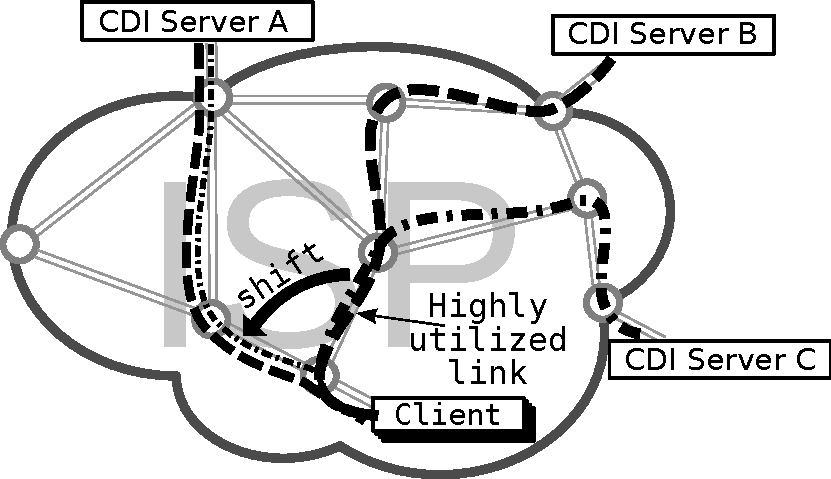
\includegraphics[width=0.90\linewidth]{figures-pdf/trafficShift-illustration}
\caption{Content-aware Traffic Engineering Process. Reprinted from \cite{Cate-CCR}. Included here by permission.}
\label{fig:Content-aware-illustration2}
\vspace{-1.5em}
\end{figure}


%%%%%%%%%%%%%%%%%%%%%%%%%%%%%%%%%%%%%%%%%%%%%%%%%%%%%%%%%%%%%%%%%%%%%%%%
\smallskip
\noindent {\bf Terminology:}\label{sec:Terminology}
%%%%%%%%%%%%%%%%%%%%%%%%%%%%%%%%%%%%%%%%%%%%%%%%%%%%%%%%%%%%%%%%%%%%%%%%
We denote as {\it flow} an OD flow between two routers in the network.  We call
a flow {\it splittable} if arbitrarily small pieces of the flow can be assigned
to other flows.  This is not to be confused with end-to-end sessions, \ie TCP
connections, which are \emph{un-splittable}.  The assumption that flows are
splittable is reasonable, as the percentage of traffic of a single end-to-end
session is small compared to that of a flow between routers. Let $C$ be the set
of nominal capacities of the links in the network $G$. We denote as {\it link
utilization} the fraction of the link capacity that is used by flows. We denote
as {\it flow utilization} the maximum link utilization among all links that a
flow traverses. We introduce the terms of {\it traffic consumer} and {\it
traffic producer} which refer to the aggregated demand of users attached to a
router, and the CDIs that are responsible for the traffic respectively. We
refer to the different alternatives from which content can be supplied by a
given CDI as \emph{network locations} that host servers.


%%%%%%%%%%%%%%%%%%%%%%%%%%%%%%%%%%%%%%%%%%%%%%%%%%%%%%%%%%%%%%%%%%%%%%%%
\ \\\noindent\textbf{Definition of CaTE:}\label{sec:CaTE-Definitions}\\\noindent
%%%%%%%%%%%%%%%%%%%%%%%%%%%%%%%%%%%%%%%%%%%%%%%%%%%%%%%%%%%%%%%%%%%%%%%%
We revisit traffic engineering by focusing on the traffic demands rather than
changing the routing.

\noindent \textbf{Definition 1: Content-aware Traffic Engineering(\cate)} is
the process of adjusting the traffic demand vector {\bf x}, given a routing
matrix $A$, so as to change the link traffic {\bf y}.

Not all the traffic can be adjusted arbitrarily. Only traffic for which
location diversity is available can be adjusted by \cate.  Therefore, {\bf
  x}={\bf x$_r$}+{\bf x$_s$} where {\bf x$_r$} denotes the content demands that
can be adjusted and {\bf x$_s$} denotes the content demands that can not be
adjusted as there is only a single location in the network where the content
can be downloaded from.  The amount of traffic that can be adjusted depends on
the diversity of locations from which the content can be obtained.  We can
rewrite the relation between traffic counts on links and traffic counts in
flows as follows: {\bf y}=$A$({\bf x$_s$} $+$ {\bf x$_r$}).  \cate adjusts the
traffic on each link of the network by adjusting the content demands {\bf
  x$_r$}: {\bf y$_r$}=$A${\bf x$_r$}. Applying \cate means adjusting the
content demand to satisfy a traffic engineering goal.


\noindent \textbf{Definition 2: Optimal Traffic Matrix} is the new traffic
matrix, {\bf x}$^*$, after applying \cate, given a network topology $G$, a
routing matrix $A$ and an initial traffic matrix {\bf x}.

Figure~\ref{fig:Content-aware-illustration2} illustrates the \cate process.  A
content consumer requests content that three different servers can deliver. Let
us assume that, without \cate, the CDI redirects the clients to servers B and
C.  Unfortunately, the resulting traffic crosses a highly-utilized link. With
\cate, content can also be downloaded from server A, thus, the traffic within
the network is better balanced as the highly utilized link is circumvented.

Minimizing the maximum utilization across all links in a network is a popular
traffic engineering goal~\cite{FT00,FT01,ImprovingPerformanceInternet2009}.  It
potentially improves the quality of experience and postpones the need for
capacity increase. \cate mitigates bottlenecks and minimizes the maximum link
utilization by re-assigning parts of the traffic traversing heavily loaded
paths. Thus it redirects traffic to other, less utilized paths.  Later in this
chapter, we will elaborate in Section~\ref{sec:impact}, different metrics such
as path length or network delay can also be used in \cate.


%%%%%%%%%%%%%%%%%%%%%%%%%%%%%%%%%%%%%%%%%%%%%%%%%%%%%%%%%%%%%%%%%%%%%%%%%
\ \\\noindent\textbf{CaTE and Traditional TE:}\label{sec:CaTE-TE}\\\noindent
%%%%%%%%%%%%%%%%%%%%%%%%%%%%%%%%%%%%%%%%%%%%%%%%%%%%%%%%%%%%%%%%%%%%%%%%%
\cate is complementary to routing-based traffic engineering as it does not
modify the routing. Routing-based traffic engineering adjusts routing weights
to adapt to traffic matrix changes. To avoid micro-loops during IGP
convergence~\cite{transient-IGP}, it is common practice to only adjust a small
number of routing weights~\cite{FT01}. To limit the number of changes in
routing weights, routing-based traffic engineering relies on traffic matrices
computed over long time periods and offline estimation of the routing weights.
Therefore, routing-based traffic engineering operates on time scales of hours,
which can be too slow to react to rapid change of traffic demands.  \cate
complements routing-based traffic engineering and can influence flows at
shorter time scales by assigning clients to servers on a per request
basis. Thus, \cate influences the traffic within a network online in a
fine-grained fashion.


%%%%%%%%%%%%%%%%%%%%%%%%%%%%%%%%%%%%%%%%%%%%%%%%%%%%%%%%%%%%%%%%%%%%%%%%
\ \\\noindent\textbf{CaTE and Multipath Routing:}\label{sec:CaTE-Multipath}\\\noindent
%%%%%%%%%%%%%%%%%%%%%%%%%%%%%%%%%%%%%%%%%%%%%%%%%%%%%%%%%%%%%%%%%%%%%%%%
Multipath routing helps end-hosts to increase and control their upload
capacity~\cite{PathSelection:CACM2011}. It can be used to minimize transit
costs~\cite{Optimizing:Goldenberg2004}. Multipath also enables ASes to
dynamically distribute the load inside networks in the presence of volatile and
hard to predict traffic demand
changes~\cite{TrafficDemand:ToN2001,MATE2001,TeXCP,Replex}.  This is a
significant advantage, as routing-based traffic engineering can be too slow to
react to phenomena such as flash crowds. Multipath takes advantage of the
diversity of paths to better distribute traffic.

\cate also leverages the path diversity, and can be advantageously combined
with multipath to further improve traffic engineering and end-user
performance. One of the advantages of \cate is its limited investments in
hardware deployed within an ISP. It can be realized with no change to routers,
contrary to some of the previous multipath
proposals~\cite{TeXCP,MATE2001,Replex}.  The overhead of \cate is also limited
as no state about individual TCP connections needs to be maintained, contrary
to multipath~\cite{TeXCP,MATE2001,Replex}.  In contrast
to~\cite{MATE2001,TeXCP}, \cate is not restricted to MPLS-like solutions and is
easily deployable in today's networks.


%%%%%%%%%%%%%%%%%%%%%%%%%%%%%%%%%%%%%%%%%%%%%%%%%%%%%%%%%%%%%%%%%%%%%%%%
\ \\\noindent\textbf{CaTE and Oscillations:}\label{sec:CaTE-Oscilations}\\\noindent
%%%%%%%%%%%%%%%%%%%%%%%%%%%%%%%%%%%%%%%%%%%%%%%%%%%%%%%%%%%%%%%%%%%%%%%%
Theoretical results~\cite{AdaptiveRouting2005,Convergence:Fischer2006} have shown that
load balancing algorithms can take advantage of multipath while provably avoiding traffic
oscillations. In addition, their convergence is fast. Building on these theoretical results, Fischer
et al. proposed REPLEX~\cite{Replex}, a dynamic traffic engineering algorithm that exploits
the fact that there are multiple paths to a destination. It dynamically changes the traffic load
routed on each path. Extensive simulations show that REPLEX leads to fast convergence, without
oscillations, even when there is lag between consecutive updates about the state of the network.
\cate is derived from the same principles and thus inherits all the above-mentioned desired properties.



%%%%%%%%%%%%%%%%%%%%%%%%%%%%%%%%%%%%%%%%%%%%
\subsubsection{Potential of Collaboration}\label{sec:impact}
%%%%%%%%%%%%%%%%%%%%%%%%%%%%%%%%%%%%%%%%%%%%

In this section, we quantify the potential benefits of \cate when deployed
within an European Tier-1 ISP using operational data.

%%%%%%%%%%%%%%%%%%%%%%%%%%%%%%%%%%%%%%%%%%%%%%%%%%%%%%%%
\noindent\textbf{Experimental Setting:}\label{sec:Experimental-Setting}
%%%%%%%%%%%%%%%%%%%%%%%%%%%%%%%%%%%%%%%%%%%%%%%%%%%%%%%
To evaluate \cate, an understanding of the studied ISP network is necessary,
including its topological properties and their implications on the flow of
traffic.  Indeed, the topological properties of the ISP network influence the
availability of disjoint paths, which are key to benefit from the
load-balancing ability of \cate.  Because \cate influences traffic aggregates
inside the ISP network at the granularity of requests directed to CDIs,
fine-grained traffic statistics are necessary.  Traffic counts per-OD flow,
often used in the literature, are too coarse an input for \cate.

%%%%%%%%%%%%%%%%%%%%%%%%%%%%%%%%%%%%%%%%%%%%%%%%%%%%%%%%
\noindent\textbf{Data from a Large European ISP:}\label{sec:Residential-Traces}
%%%%%%%%%%%%%%%%%%%%%%%%%%%%%%%%%%%%%%%%%%%%%%%%%%%%%%%
To build fine-grained traffic demands, we rely on anonymized packet-level
traces of residential DSL connections from a large European Tier-1 ISP,
henceforth called \emph{ISP1}. For ISP1, we have the complete annotated
router-level topology including the router locations as well as all public and
private peerings. ISP1 contains more than $650$ routers and $30$ peering points
all over the world.  Using the same monitoring infrastructure as in
Section~\ref{sec:traces}, we collect a $10$ days long trace of HTTP and DNS
traffic starting on May 7, 2010. We observe 720 million DNS messages as well as
more than 1 billion HTTP requests involving about 1.4 million unique hostnames,
representing more than 35 TBytes of data. We note that more than 65\% of the
traffic volume is due to HTTP.

A large fraction of the traffic in the Internet is due to large CDIs, including
CDNs, hyper-giants, and OCHs, as reported in earlier
studies~\cite{TrafficTypesGrowth:2011,arbor,PADIS2010}. In
Figure~\ref{fig:CDF-Traffic-CPs}, we plot the cumulative fraction of HTTP
traffic volume as a function of the CDIs that originate the traffic. For this,
we regard a CDI as a organizational unit where all servers from the distributed
infrastructure serve the same content, such as Akamai or Google.  We rank the
CDIs by decreasing traffic volume observed in our trace. Note that the x-axis
uses a logarithmic scale. The top 10 CDIs are responsible for around 40\% of
the HTTP traffic volume and the top 100 CDIs for close to 70\% of the HTTP
traffic volume. The marginal increase of traffic is diminishing when increasing
the number of CDIs. This shows that collaborating directly with a small number
of large CDIs, can yield significant savings.

In Figure~\ref{fig:CPs-Total-Traffic} we plot the traffic of the top 1, 10, 100
CDIs by volume as well as the total traffic over time normalized to the peak
traffic in our dataset.  For illustrative purposes, we show the evolution
across the first $60$ hours of our trace. A strong diurnal pattern of traffic
activity is observed. We again observe that a small number of CDIs are
responsible for about half of the traffic. Similar observations are made for
the rest of the trace.

\begin{figure}[tbp]
\center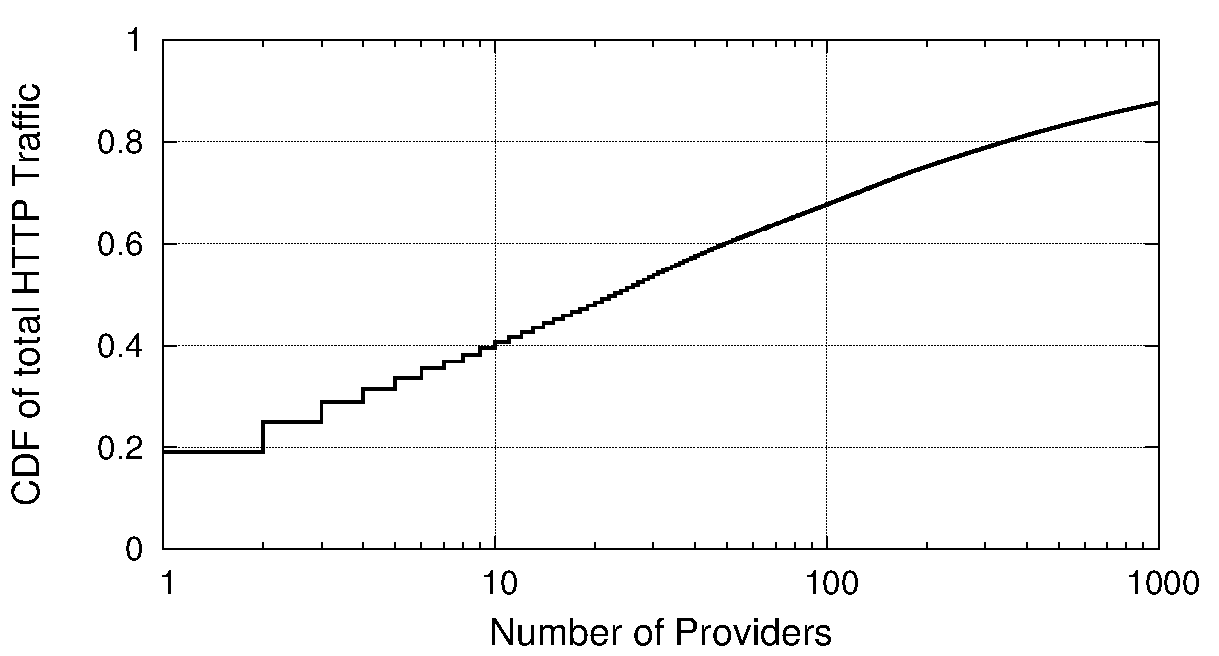
\includegraphics[width=1\linewidth]{figures-pdf/providersVsVolume}
\caption{CDF of traffic volume of CDIs in ISP1. Reprinted from \cite{Cate-CCR}. Included here by permission.}
\label{fig:CDF-Traffic-CPs}
\vspace{-1.5em}
\end{figure}


\begin{figure}[tbp]
\center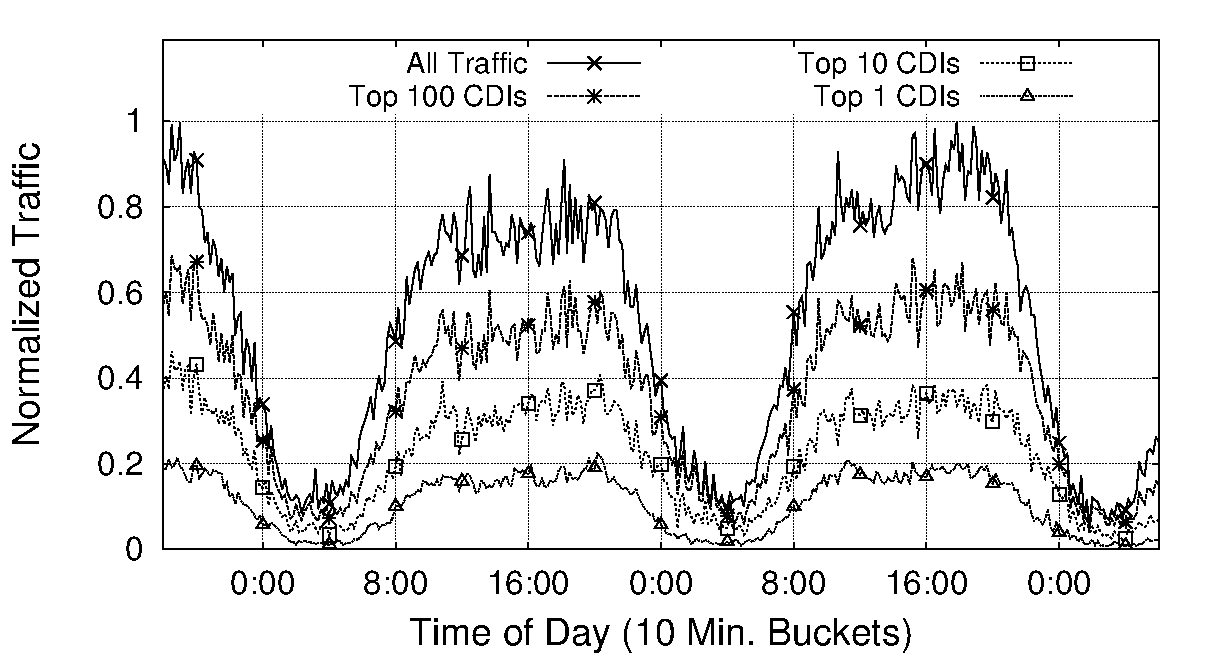
\includegraphics[width=1\linewidth]{figures-pdf/Volume_timeseries}
\caption{Normalized traffic for top CDIs by volume in ISP1. Reprinted from \cite{Cate-CCR}. Included here by permission.}
\label{fig:CPs-Total-Traffic}
\vspace{-1.5em}
\end{figure}



%%%%%%%%%%%%%%%%%%%%%%%%%%%%%%%%%%%%%%%%%%%%%%%%%%%%%%%%%%%%%%%%%%%%%%%%%%%%%%%%%%%
\noindent\textbf{Understanding the Location Diversity of CDIs:}\label{sec:Traffic-by-Content-Provider}
%%%%%%%%%%%%%%%%%%%%%%%%%%%%%%%%%%%%%%%%%%%%%%%%%%%%%%%%%%%%%%%%%%%%%%%%%%%%%%%%%%%
To achieve traffic engineering goals, it is crucial to also understand the
location diversity of the top CDIs, as \cate relies on the fact that the same
content is available at multiple locations.  Traffic originated from multiple
network locations by a given CDI is seen by \cate as a single atomic traffic
aggregate to be engineered. Furthermore, as routing in the Internet works per
prefix, we assume that the granularity of subnets is the finest at which \cate
should engineer the traffic demand. Thus, we differentiate candidate locations
of CDIs by their subnets and quantify the location diversity of CDIs through the
number of subnets from which content can be obtained.

We examine the amount of location diversity offered by CDIs based on traces from
ISP1.  To identify the subnets of individual CDIs, we rely on a similar
methodology to the one from Poese \etal~\cite{PADIS2010}. Our granularity is
comparable to their "infrastructure redirection
aggregation". Figure~\ref{fig:VolumeChoices} shows the cumulative fraction of
HTTP traffic as a function of the number of subnets (logarithmic scale) from
which a given content can be obtained, over the entire $10$ days of the
trace. We observe that more than $50\%$ of the HTTP traffic can be delivered
from at least $8$ different subnets, and more than $60\%$ of the HTTP traffic
from more than $3$ locations. These results confirm the observations made
in~\cite{PADIS2010}.


\begin{figure}[tbp]
\center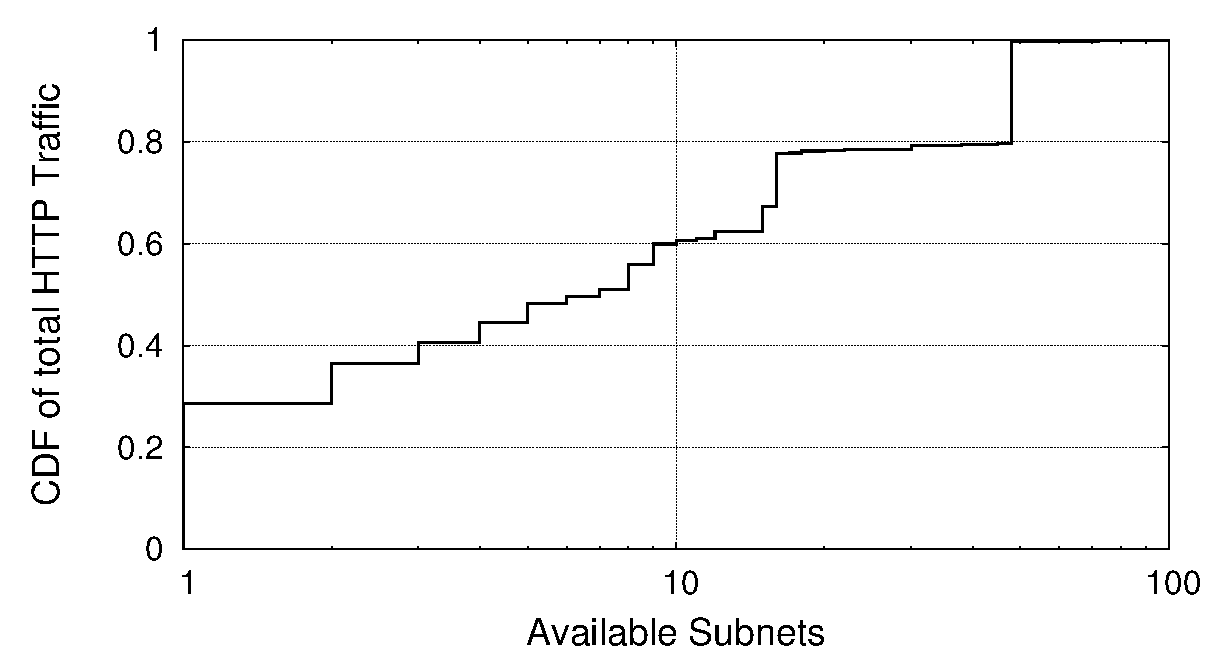
\includegraphics[width=1\linewidth]{figures-pdf/subnetVsVolumeBucket}
\caption{Subnet diversity from which content is available.}
\label{fig:VolumeChoices}
\vspace{-1.5em}
\end{figure}



%%%%%%%%%%%%%%%%%%%%%%%%%%%%%%%%%%%%%%%%%%%%%%%%%%%%%%%%%%%%%%
\noindent\textbf{Dynamics in Location Diversity:}\label{sec:Server-Dynamics}
%%%%%%%%%%%%%%%%%%%%%%%%%%%%%%%%%%%%%%%%%%%%%%%%%%%%%%%%%%%%%%
So far the location diversity of CDIs has been evaluated irrespective of time.
To complement the finding, we turn our attention to the location diversity
exposed by CDIs at small time-scales, \ie in the order of minutes.  To this
end, we split the original trace into $10$ minutes bins.
Figure~\ref{fig:TemporalEffect} shows the evolution of the number of exposed
subnets of five of the top 10 CDIs by volume.  Note that the diversity exposed
by some CDIs exhibits explicit time of day patterns, while others do not. This
can be due to the structural setup or the type of content served by the CDI.
The exposed location diversity patterns, \ie flat or diurnal, are
representative for all CDIs with a major traffic share in our trace. We
conclude that a significant location diversity is exposed by popular CDIs at
any point in time, and is quite extensive during the peak hour.

\begin{figure}[tbp]
\center
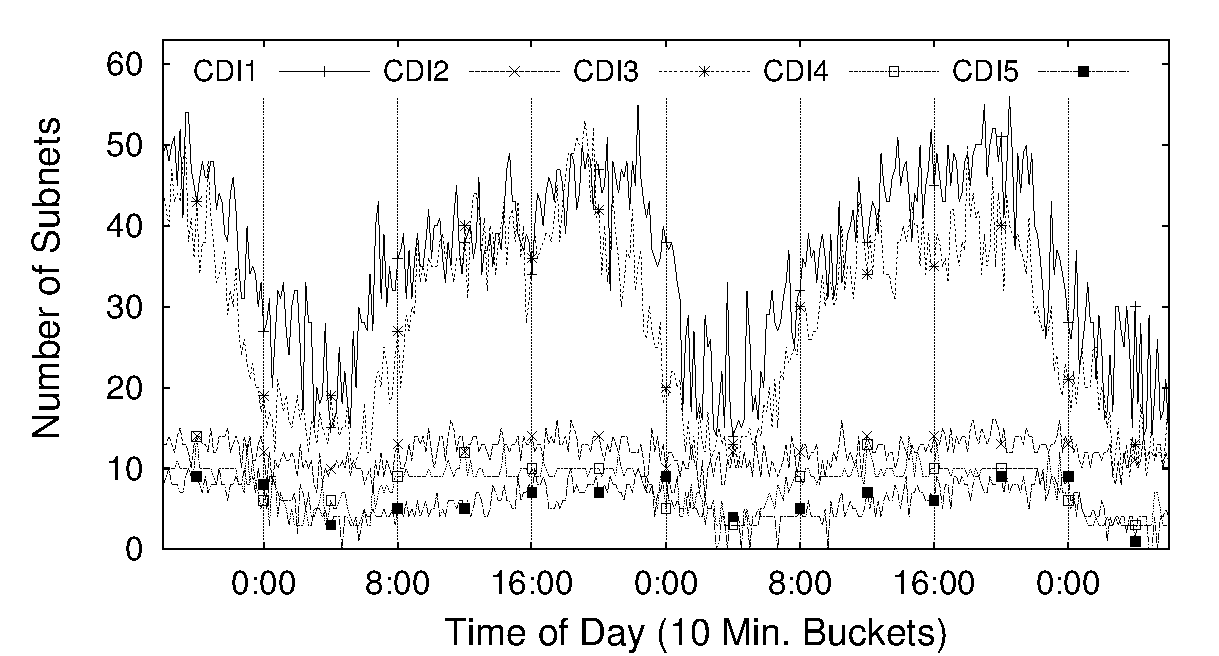
\includegraphics[width=1\linewidth]{figures-pdf/SubnetChoice_r-2}
\caption{Evolution over time of number of subnets for selected CDIs in
  the top 10 CDIs. Reprinted from \cite{Cate-CCR}. Included here by permission.}
\label{fig:TemporalEffect}
\vspace{-1.5em}
\end{figure}



%%%%%%%%%%%%%%%%%%%%%%%%%%%%%%%%%%%%%%%%%%%%%%
\noindent\textbf{Content Demand Generation:}\label{sec:TM}
%%%%%%%%%%%%%%%%%%%%%%%%%%%%%%%%%%%%%%
The location diversity is not a mere observation about CDIs deployment. It
requires to revisit the mapping between a given content demand and the realized
traffic matrix. Given the location diversity for content, multiple traffic
matrices can be realized from a given content demand. The standard view of the
OD flows therefore provides an incomplete picture of the options available for
\cate.

As an input for \cate, we introduce an abstraction of the demand that reflects
the available location diversity.  We rely on the notion of \emph{potential
  vectors}, that were denoted as $x_{r}$ in Section~\ref{sec:CaTE-Definitions}.
To generate the potential vector for a given CDI, the amount of traffic this CDI
originates as well as the potential ingress points need to be known. Combining
all potential vectors and $x_{s}$, we synthesize a network-wide content demand
matrix for each time bin, by scaling the traffic demand to match the network
utilization of ISP1.  For our evaluation, we use the series of content demand
matrices over a period of $10$ days. The content demands are based exclusively
on the HTTP traffic of our trace.


\subsection{Summary}

In this section we presented the potential of the \emph{Oracle} and
\emph{Content-aware Traffic Engineering} (\cate), two collaborative approach to
improve content delivery while achieving traffic engineering goals.  Both
leverage location diversity offered by P2P systems or CDIs. Moreover, \cate
enables dynamic adaption to traffic demand shifts. With \cate/the oracle the
decision on end-user to server/peer assignment can be done jointly between the
CDI/P2P system and the ISP.  Our analysis of operational data from a European
Tier-1 ISP has shown ample opportunities for \cate to improve content delivery
as it is done today.

Through extensive experiments, we show that both P2P users and ISPs benefit
from ISP-aided P2P locality, measured in terms of improved content download
times, increased network locality of query responses and desired content, and
overall reduction in P2P traffic. For a more detailed analysis of the possible
improvements and additional background information on the parameter set and
resulting improvements, we refer the reader to~\cite{afs-cispp2pcip-ccr07,A-IANSPS-08}.

In~\cite{Cate-CCR, CaTE-TR, Sigmetrics2012} we quantify the benefits of \cate
and consider one of the most popular traffic engineering goals, namely
minimizing the maximum utilization of the links in the
network~\cite{FT00,FT01}.  Our evaluation shows that \cate yields encouraging
results, even when only a few large CDIs are collaborating with an ISP. In fact,
even metrics that are not directly related to the optimization function of
\cate are improved. Besides significant improvements for the operation of ISP
networks, the end-users to also benefit from these gains. This can be
attributed to the decrease of delay as well as the reduced link
utilization. In~\cite{CaTE-TR} we also consider other network metrics such as
path length or path delay and the effect of other network topologies.  We also
outline how \cate can aid in the deployment of popular large scale
applications, \eg NetFlix, by selecting strategic locations for caches and
specific optimization goals to support their operation. With this we conclude
the section on collaborative traffic engineering and continue to elaborate on
our idea for ``in-network server deployment'' in the next chapter.

